\section{Merging Heuristics}
\indent Unfortunately, although the label-swapping algorithm yields perfectly satisfying graphs, it often doesn't sufficiently disguise a given graph.  In this section, we present a heuristic, called \emph{adjacency group merges} (or simply \emph{merges}) that further randomizes a given graph, but is not guaranteed to maintain the same k-neighborhood. There are two versions of this heuristic that we developed, \emph{deterministic merges} and \emph{non-deterministic merges}.

\begin{dfn}
\noindent A \emph{merge} or \emph{merging} of a graph's adjacency groups combines similar adjacency groups into larger groups containing the union of their nodes based on their \emph{difference}. It runs deterministically and maps every pair of nodes to  the differencence value between their adjacency groups and merges adjacency groups of the first n that have not been involved in a previous merge. \\
\end{dfn}

\begin{dfn}
The \emph{difference} between adjacency groups $A$ and $B$ is the size of the symmetric difference of $N_k(v)$ and $N_k(u)$, for $v \in A$ and $u \in B$. 
\end{dfn}

\begin{figure}[htb]
	\begin{algorithmic}
		\renewcommand{\algorithmicrequire}{\textbf{Input:}}
		\renewcommand{\algorithmicensure}{\textbf{Output:}}
		\Require {graph $G=(V,E)$, k-neighborhoods $K= \{k_{1}, k_{2}, ...\}$, adjecency groups $A=\{a_{1}, a_{2}, ...\}$, limit L}
		\Ensure {adjecency groups $A'$}
		\ForAll {$v \in V$}
			\ForAll {$w \in W$ where $v \neq w$}
				\State {find $Diff(A(v),A(w))$}
			\EndFor
		\EndFor
		\ForAll {$(v,w,d) \in V \times V \times {\mathbb Z}$ sorted by $d = Diff(A(v),A(w))$ where $v \neq w$}
			\State {$n = 0$}
		\EndFor
		\If {$A(v)$ has not been merged and $A(w)$ has not been merged}
			\State {$merge(A(v),A(w))$}
			\State {mark $A(v)$ as merged}
			\State {mark $A(w)$ as merged}
			\State {$n++$}
			\If {$n = L$}
				\State {break}
			\EndIf
		\EndIf
	\end{algorithmic}
	\caption{Pseudocode for the Deterministic Merging Heuristic Algorithm.}
	\label{fig:deterministic-merging}
\end{figure}

\indent The results from LinkedIn data show that with a low value of $k$, such as $k=2$, there are far fewer repeated original edges than without the merging heuristic; however, there is a large number of invalid edges in the masked graph. With the value of $k$ increased to $3$, the number of repeated edges stays the same, and there are far fewer invalid new edges. This is a very good masking of the original graphs while still mostly maintaining the correct k-neighborhoods. \\

\begin{figure}[ht]
  \centering
  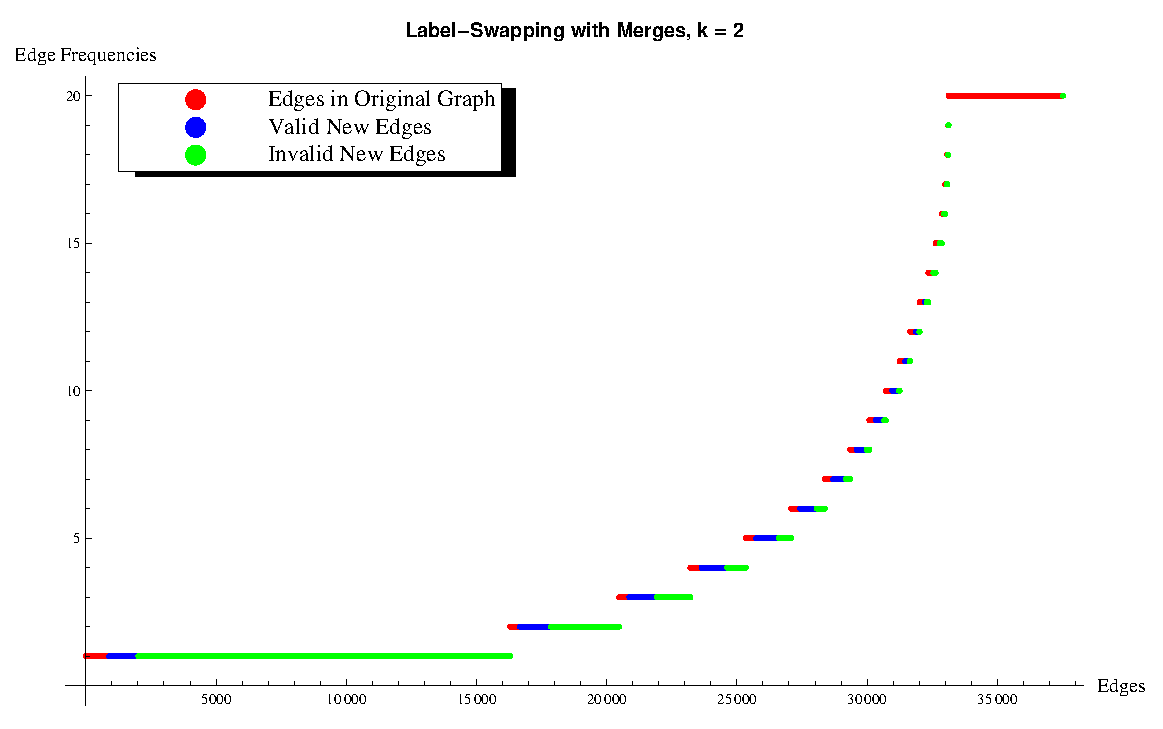
\includegraphics[scale=0.8 ]{s40_k_2_det_graph.eps}
  \caption{The results from the label-swapping algorithm when run 20 times on the blog data when k=2. Adjacency groups differing by 5 or less were merged.}
  \label{fig:s40-k=2-merge}
\end{figure}

\begin{figure}[ht]
  \centering
  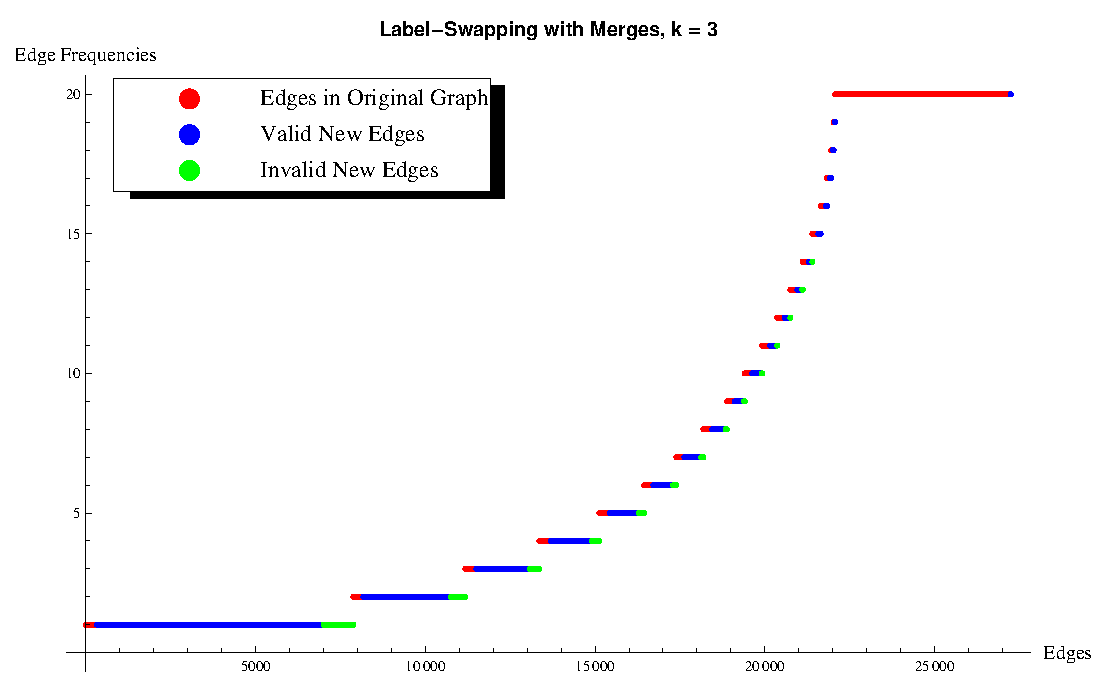
\includegraphics[scale=0.8]{s40_k_3_det_graph.eps}
  \caption{The results from the label-swapping algorithm when run 20 times on the blog data when k=3. Adjacency groups differing by 5 or less were merged.}
  \label{fig:s40-k=3-merge}
\end{figure}
